%%%%%%%%%%%%%%%%%%%%%%%%%%%%%%%%%%%%%%%%%%%%%%%%%%%%%
% Author: [Francesco Giraudo]
% Date: 2025-06-02
% Description: [Final Project - Computational Finance]
%%%%%%%%%%%%%%%%%%%%%%%%%%%%%%%%%%%%%%%%%%%%%%%%%%%%%


\documentclass{article}
\usepackage[english]{babel}
\usepackage{amsfonts}
\usepackage{amsmath} 
\usepackage{amssymb}
\usepackage{graphicx}
\usepackage{geometry}
\usepackage{mdframed}
\usepackage{booktabs}
\usepackage{geometry}
\usepackage{float}

\geometry{a4paper, margin=1in}

% Set custom margins
\geometry{
  top=0.8in,
  bottom=0.8in,
  left=0.75in,
  right=0.75in
}

% Eliminate paragraph indentation
\setlength{\parindent}{0pt}

\title{Computational Finance - Final project: Convertible Bonds}
\author{Francesco Giraudo \\ \small{Vrije Universiteit} \\ {\small\texttt{f.giraudo@student.vu.nl}}}
\date{\today}

\begin{document}

\maketitle

\bigskip

\section*{Introduction}

Convertible bonds are hybrid financial instruments that combine features of both debt and equity. They pay regular coupon payments and return the principal at maturity, similar to traditional bonds. However, they also grant the bondholder the option to convert the bond into a predetermined number of shares of the issuing company at specific times before maturity. The option to convert allows bondholders to participate in the equity upside while offering downside protection through the bond's principal and coupon payments. Convertible bonds are typically less volatile than stocks but offer higher returns than regular bonds.  \\

In this report I will use the following notation:
\begin{itemize}
    \item $N$ : Face value of the bond,
    \item $K$ : Annual coupon rate,
    \item $T$ : Maturity time (years),
    \item $\ell$ : Conversion ratio (number of shares per bond),
    \item $r$ : Risk-free interest rate,
    \item $\sigma$ : Volatility of the underlying stock,
    \item $S(t)$ : Stock price at time $t$.
\end{itemize}

\bigskip

\section{Backward Induction for Convertible Bond Pricing}


\subsection{Mathematical Formulation}

The bondholder has the option to convert the bond into shares only at specific discrete times:
\begin{itemize}
    \item After each coupon payment date $t_i$,
    \item At final maturity $T$.
\end{itemize}

I assume the stock price $S(t)$ follows a stochastic process under the risk-neutral measure. Define $V(t, S)$ as the value of the convertible bond at time $t$ when the stock price is $S$.

The dynamic programming (backward induction) recursion is formulated as follows:
\begin{itemize}
    \item \textbf{At maturity} $T$:
    \begin{equation}
        V(T, S) = \max\left( N, \ell S \right),
    \end{equation}
    reflecting the choice between receiving the bond's face value or converting into shares at maturity.
    
    \item \textbf{At coupon payment dates} $t_i$:
    \begin{equation}
        V(t_i, S) = \max \left\{
            e^{-r \Delta t} \mathbb{E} \left[ V(t_{i+1}, S') \mid S(t_i) = S \right] + c N \Delta t, \;
            \ell S
        \right\},
    \end{equation}
    where:
    \begin{itemize}
        \item $\mathbb{E}[\cdot]$ denotes the risk-neutral expectation,
        \item $K N \Delta t$ is the coupon payment received at $t_i$.
    \end{itemize}
    
    \item \textbf{At non-coupon payment dates} (no conversion allowed):
    \begin{equation}
        V(t, S) = e^{-r \Delta t} \mathbb{E} \left[ V(t + \Delta t, S') \mid S(t) = S \right].
    \end{equation}
\end{itemize}

At each coupon date and at maturity, the bondholder optimally chooses between:
\begin{itemize}
    \item Continuing to hold the bond (receiving future coupon payments and principal at maturity),
    \item Early conversion into shares.
\end{itemize}

\vspace{0.3cm}
\noindent
The expectation $\mathbb{E}[\cdot]$ is evaluated using a binomial tree discretization of the stock price dynamics under the risk-neutral measure and Monte-Carlo methods.

\subsection{Binomial Trees Method}

To solve the dynamic programming recursion, the time interval $[0, T]$ is discretized into $N_{\text{steps}}$ steps of size $\Delta t = T / N_{\text{steps}}$. A finer grid is used with monthly steps, while conversion opportunities are restricted to semiannual coupon dates. A binomial tree is constructed to model the evolution of the stock price $S(t)$. \\ At each time step:
\begin{itemize}
    \item The stock price can move up by a factor $u = e^{\sigma \sqrt{\Delta t}}$ or down by a factor $d = 1/u$.
    \item The risk-neutral probability $p$ of an upward move is given by:
    \begin{equation}
        p = \frac{e^{r \Delta t} - d}{u - d}.
    \end{equation}
\end{itemize}

At each node:
\begin{itemize}
    \item The \textbf{continuation value} is computed as the discounted expected value of future bond values plus coupon payments (if at a coupon date):
    \begin{equation}
        \text{Continuation Value} = e^{-r \Delta t} \left( p V_{\text{up}} + (1 - p) V_{\text{down}} \right) + K N \Delta t.
    \end{equation}
    \item The \textbf{conversion value} is:
    \begin{equation}
        \text{Conversion Value} = \ell S.
    \end{equation}
\end{itemize}

At coupon dates:
\begin{equation}
    V(t_i, S) = \max \left( \text{Continuation Value}, \text{Conversion Value} \right),
\end{equation}
and at non-coupon dates, only continuation is allowed:
\begin{equation}
    V(t, S) = \text{Continuation Value}.
\end{equation}

At maturity:
\begin{equation}
    V(T, S) = \max(N, \ell S).
\end{equation}


The following parameters are used for the numerical simulation:
\begin{itemize}
    \item Initial stock price: $S_0 = 200$
    \item Face value: $N = 1000$
    \item Conversion ratio: $\ell = 3$
    \item Annual coupon rate: $K_{\text{coupon}} = 0.016$
    \item Risk-free rate: $r = 0.03$
    \item Volatility: $\sigma = 0.3$
    \item Maturity: $T = 5$ years
    \item Number of time steps: $N_{\text{steps}} = 60$ (monthly steps)
\end{itemize}

\begin{figure}[h!]
    \centering
    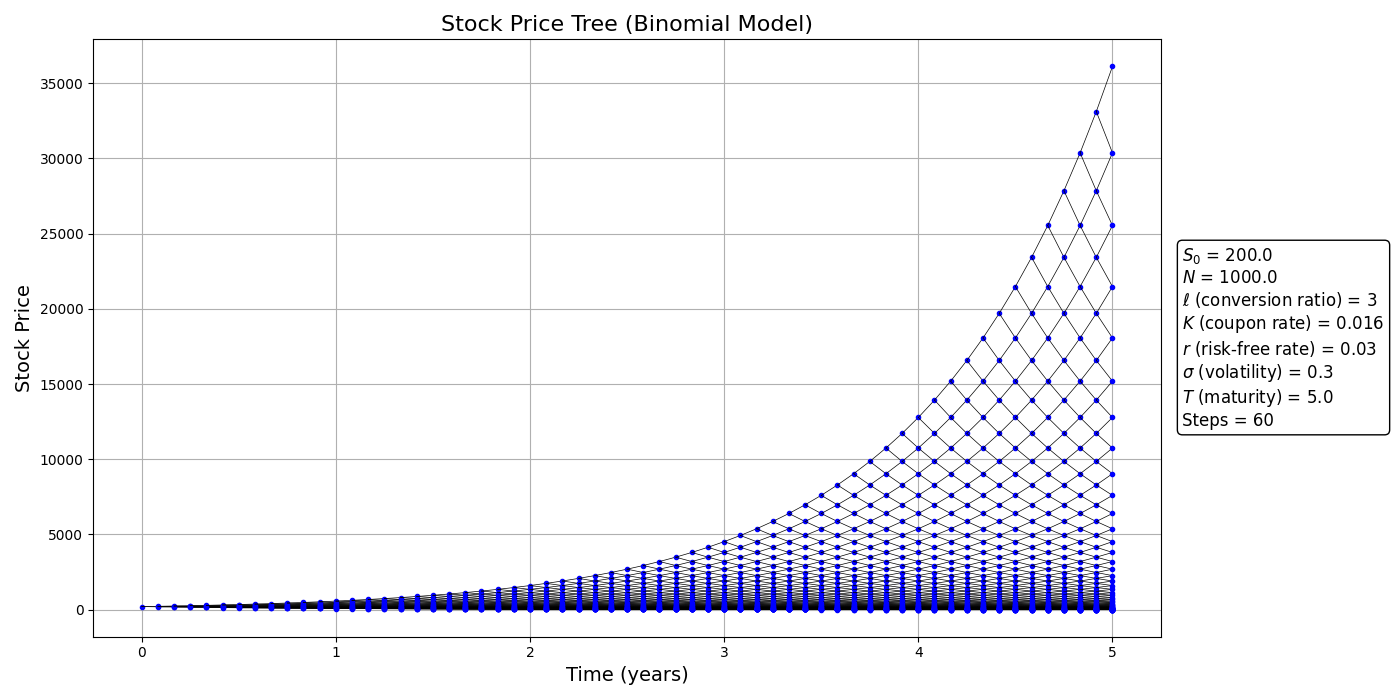
\includegraphics[width=0.65\linewidth]{13_ConvertibleBonds/img/01_StockPrice.png}
    \caption{Stock Price Tree (Binomial Model)}
    \label{fig:01_stock_price}
\end{figure}


\begin{figure}[h!]
    \centering
    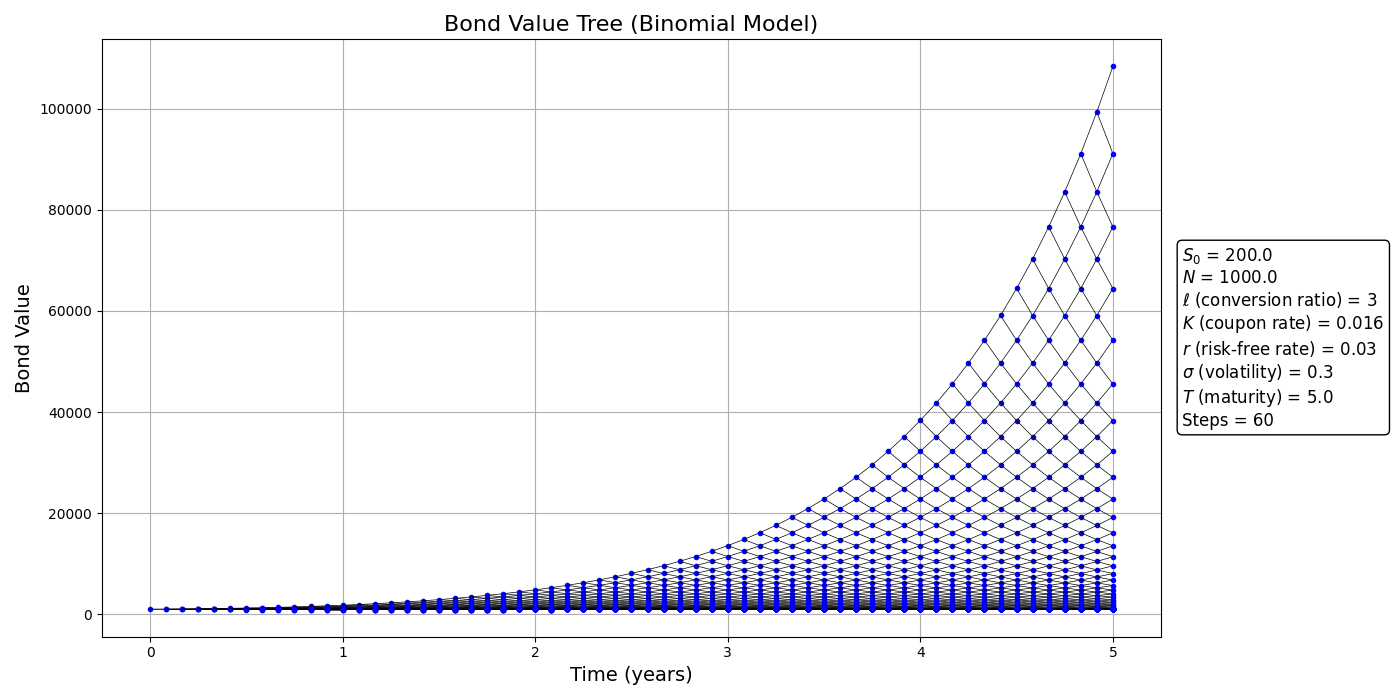
\includegraphics[width=0.65\linewidth]{13_ConvertibleBonds/img/01_BondValue.png}
    \caption{Bond Value Tree (Binomial Model)}
    \label{fig:01_bonds_price}
\end{figure}


Using the binomial tree method with the above parameters, the computed price of the convertible bond at $t = 0$ is:
\begin{equation}
    V(0, S_0) = 1014.16
\end{equation}



\section{Regression Monte Carlo for Convertible Bond Pricing}

\subsection{Mathematical Formulation}

The Regression Monte Carlo (RMC) approach for pricing convertible bonds is based on the Longstaff-Schwartz algorithm. This method uses simulation paths and regression to estimate continuation values, allowing for efficient pricing of early exercise features.

At each potential conversion date, the bondholder must decide whether to convert by comparing:
\begin{itemize}
    \item The immediate conversion value: $\ell S(t)$
    \item The continuation value: $\mathbb{E}[V(t+\Delta t, S(t+\Delta t)) | S(t)]$
\end{itemize}

The algorithm proceeds as follows:

\begin{enumerate}
    \item Generate $N$ paths of the stock price process under the risk-neutral measure:
    \begin{equation}
        dS(t) = rS(t)dt + \sigma S(t)dW(t)
    \end{equation}
    
    \item Initialize terminal cash flows at maturity $T$:
    \begin{equation}
        V_i(T) = \max(N, \ell S_i(T)) \quad \text{for } i = 1, 2, \ldots, N
    \end{equation}
    
    \item Working backward in time, at each potential conversion date $t_j$:
        \begin{itemize}
            \item Identify paths where conversion is in-the-money: $\ell S_i(t_j) > 0$
            \item For these paths, estimate the continuation value using regression:
            \begin{equation}
                \hat{C}_i(t_j) = \sum_{k=0}^{M} \beta_k \phi_k(S_i(t_j))
            \end{equation}
            where $\phi_k$ are basis functions (polynomials) and $\beta_k$ are regression coefficients
            \item Compare the estimated continuation value with the immediate conversion value:
            \begin{equation}
                V_i(t_j) = \max(\hat{C}_i(t_j), \ell S_i(t_j))
            \end{equation}
            \item Add coupon payments if $t_j$ is a coupon date:
            \begin{equation}
                V_i(t_j) = V_i(t_j) + K N \Delta t
            \end{equation}
            \item Discount cash flows to the previous time step:
            \begin{equation}
                V_i(t_{j-1}) = e^{-r(t_j-t_{j-1})}V_i(t_j)
            \end{equation}
        \end{itemize}
        
    \item The convertible bond price at $t=0$ is the average of discounted cash flows:
    \begin{equation}
        V(0) = \frac{1}{N}\sum_{i=1}^{N}V_i(0)
    \end{equation}
\end{enumerate}

\subsection{Implementation Results}

Using the Regression Monte Carlo approach with the same parameters, but simulating daily:
\begin{itemize}
    \item Initial stock price: $S_0 = 200$
    \item Face value: $N = 1000$
    \item Conversion ratio: $\ell = 3$
    \item Annual coupon rate: $K_{\text{coupon}} = 0.016$
    \item Risk-free rate: $r = 0.03$
    \item Volatility: $\sigma = 0.3$
    \item Maturity: $T = 5$ years
    \item Number of simulation paths: $n_{\text{paths}} = 10,000$
    \item Number of time steps: $n_{\text{steps}} = 252 \times 5$ (daily steps)
    \item Polynomial regression degree: 3
\end{itemize}

The computed price of the convertible bond at $t = 0$ is:
\begin{equation}
    V(0, S_0) = 1064.9177
\end{equation}

This represents a conversion premium of 6.49\% over the face value, reflecting the embedded option value of the conversion feature.

\begin{figure}[H]
    \centering
    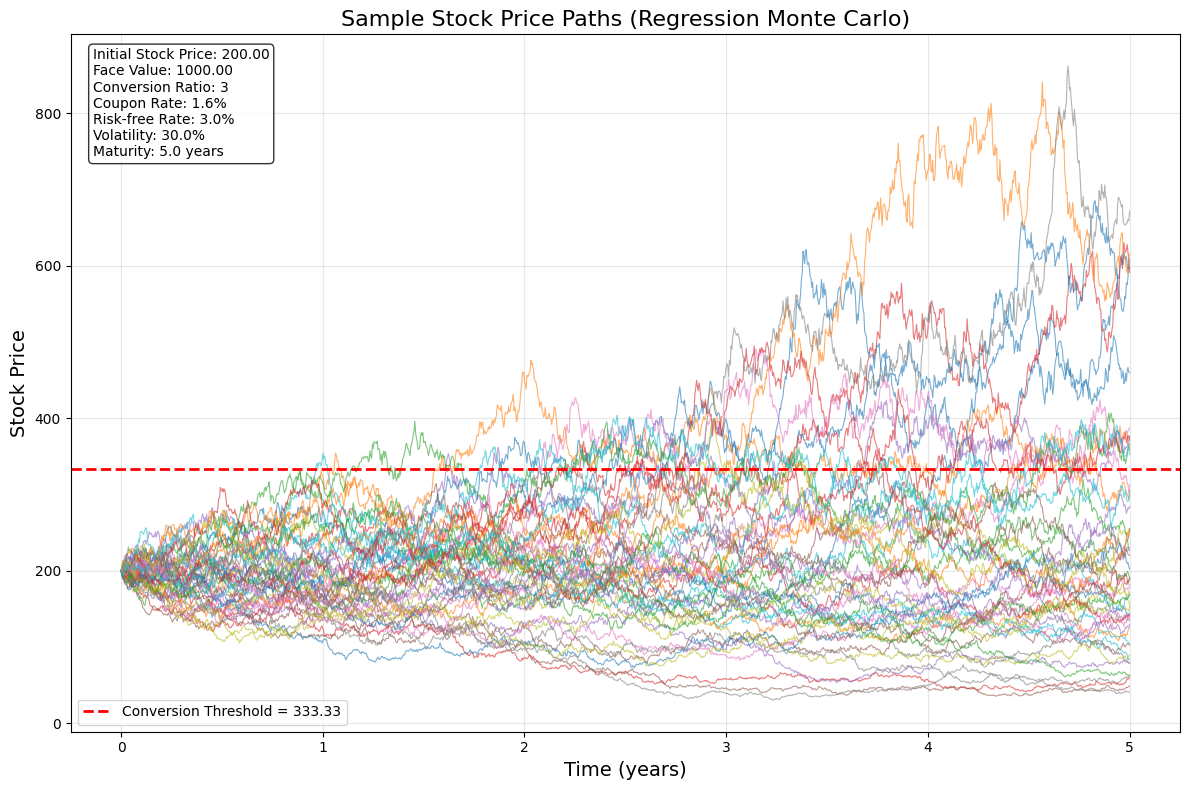
\includegraphics[width=0.75\textwidth]{img/02_sample_paths.png}
    \caption{Sample stock price paths under the risk-neutral measure. The horizontal red line represents the conversion threshold $N/\ell = 333.33$.}
    \label{fig:sample_paths}
\end{figure}

Figure \ref{fig:sample_paths} shows sample stock price paths generated under the risk-neutral measure. The horizontal red line represents the conversion threshold $N/\ell = 333.33$, which is the stock price at which the conversion value equals the face value of the bond.

\begin{figure}[H]
    \centering
    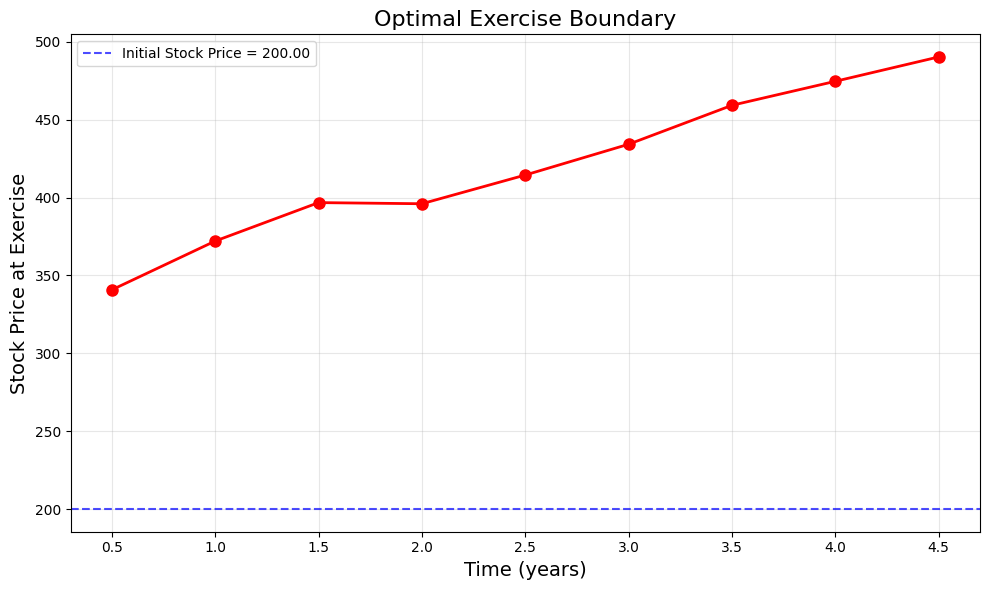
\includegraphics[width=0.75\textwidth]{13_ConvertibleBonds/img/02_optimal_exercise_bound.png}
    \caption{Optimal exercise boundary showing the stock price threshold above which early conversion is optimal at each conversion date.}
    \label{fig:exercise_boundary}
\end{figure}

\subsection{Sensitivity Analysis}

The convertible bond price is sensitive to various market parameters. Figure \ref{fig:sensitivity_analysis} illustrates how the bond price varies with volatility, stock price, and interest rate.

\begin{figure}[h!]
    \centering
    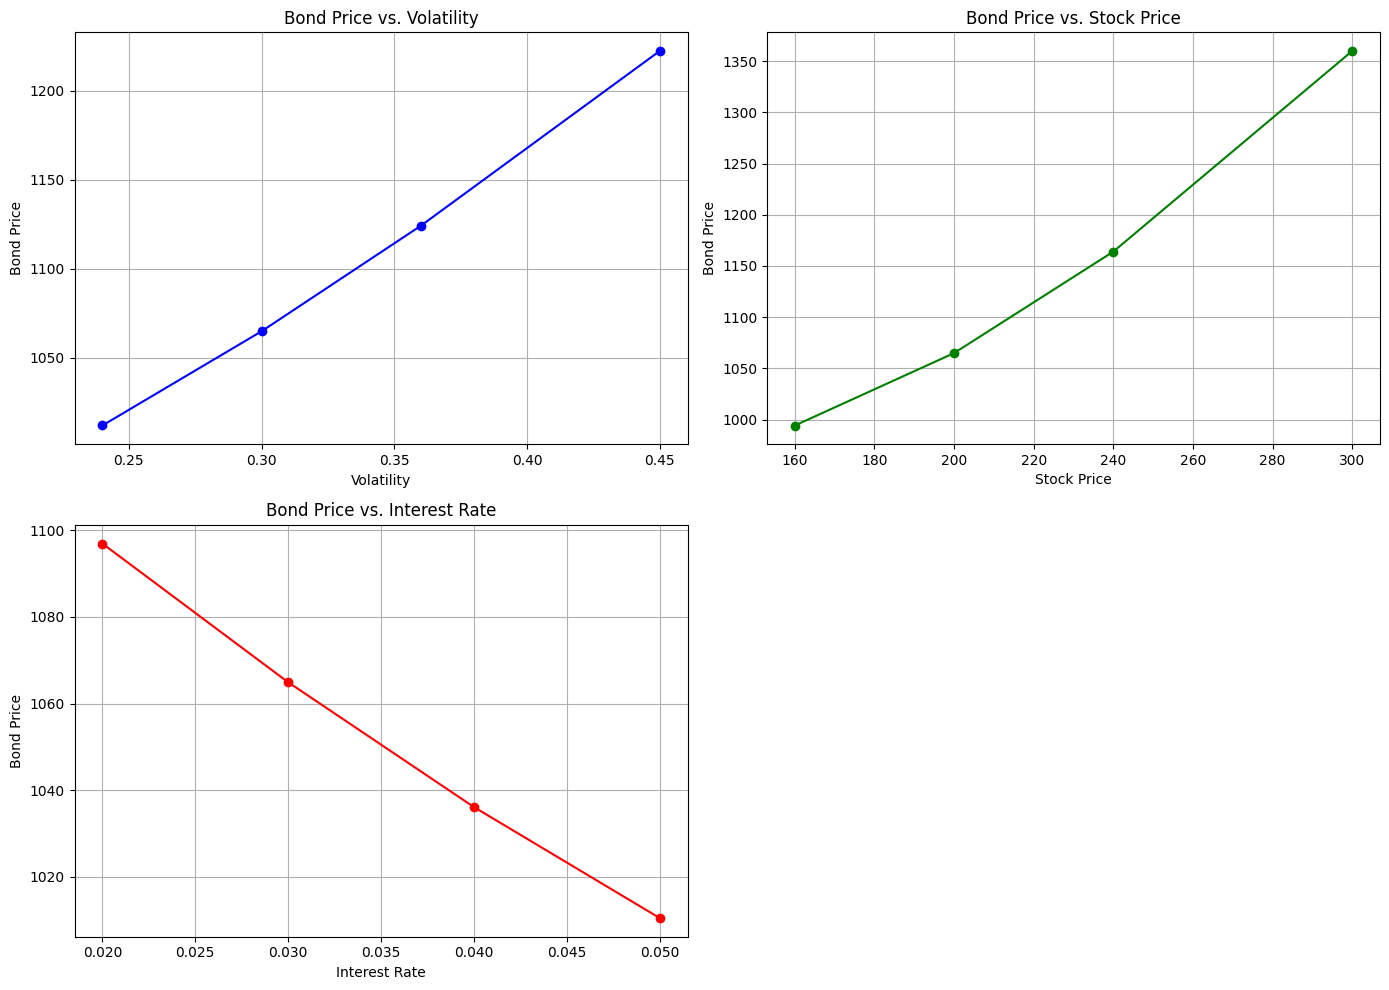
\includegraphics[width=0.8\textwidth]{13_ConvertibleBonds/img/02_sensitivity_analysis.png}
    \caption{Sensitivity of convertible bond price to volatility, stock price, and interest rate.}
    \label{fig:sensitivity_analysis}
\end{figure}

\subsubsection{Volatility Sensitivity}

Increasing volatility increases the convertible bond price, as shown in the top-left panel of Figure \ref{fig:sensitivity_analysis}. This occurs because higher volatility increases the probability of the stock price exceeding the conversion threshold, enhancing the value of the conversion option. Specifically:

\begin{itemize}
    \item At $\sigma = 24\%$: Bond price = 1011.99 ($\Delta$ = -52.93)
    \item At $\sigma = 30\%$: Bond price = 1064.92 (base case)
    \item At $\sigma = 36\%$: Bond price = 1124.17 ($\Delta$ = +59.25)
    \item At $\sigma = 45\%$: Bond price = 1222.29 ($\Delta$ = +157.37)
\end{itemize}

The relationship is non-linear, with larger increases in bond price as volatility increases, demonstrating the convex nature of the option component.

\subsubsection{Stock Price Sensitivity}

The convertible bond price is highly sensitive to the underlying stock price, as shown in the top-right panel of Figure \ref{fig:sensitivity_analysis}. Higher stock prices increase the probability of profitable conversion, thereby increasing the bond value:

\begin{itemize}
    \item At $S_0 = 160$: Bond price = 994.18 ($\Delta$ = -70.74)
    \item At $S_0 = 200$: Bond price = 1064.92 (base case)
    \item At $S_0 = 240$: Bond price = 1164.00 ($\Delta$ = +99.08)
    \item At $S_0 = 300$: Bond price = 1359.88 ($\Delta$ = +294.96)
\end{itemize}

When the stock price is low ($S_0 = 160$), the bond trades below par value, indicating that the market expects the bond to be redeemed at face value rather than converted. As the stock price increases, the bond price increases at an accelerating rate, reflecting the increasing probability of conversion.

\subsubsection{Interest Rate Sensitivity}

The convertible bond price decreases as interest rates increase, as shown in the bottom-left panel of Figure \ref{fig:sensitivity_analysis}:

\begin{itemize}
    \item At $r = 2\%$: Bond price = 1096.91 ($\Delta$ = +31.99)
    \item At $r = 3\%$: Bond price = 1064.92 (base case)
    \item At $r = 4\%$: Bond price = 1036.12 ($\Delta$ = -28.80)
    \item At $r = 5\%$: Bond price = 1010.52 ($\Delta$ = -54.40)
\end{itemize}

This negative relationship arises from two competing effects:
\begin{enumerate}
    \item Higher interest rates reduce the present value of future cash flows (coupon payments and principal), decreasing the bond component value.
    \item Higher interest rates increase the expected growth rate of the stock price under the risk-neutral measure, potentially increasing the conversion option value.
\end{enumerate}

In this case, the first effect dominates, resulting in a negative relationship between interest rates and bond price.



\section{Convertible Bonds with Arbitrary Conversion Dates}

\subsection{Mathematical Formulation}

In this section, I extend the analysis to allow for conversion at arbitrary dates, not necessarily coinciding with coupon payments. This generalization is important because real-world convertible bonds often have different conversion schedules.

Let me denote the set of allowed conversion dates as $\mathcal{T}_c = \{t_1^c, t_2^c, \ldots, t_m^c\}$, which may differ from the set of coupon payment dates $\mathcal{T}_p = \{t_1^p, t_2^p, \ldots, t_n^p\}$. The valuation problem becomes more complex as I need to track both payment and conversion events separately.

The dynamic programming recursion is modified as follows:

\begin{itemize}
    \item \textbf{At maturity} $T$:
    \begin{equation}
        V(T, S) = \max\left( N, \ell S \right)
    \end{equation}
    
    \item \textbf{At dates that are both coupon payment and conversion dates} ($t \in \mathcal{T}_p \cap \mathcal{T}_c$):
    \begin{equation}
        V(t, S) = \max \left\{
            e^{-r \Delta t} \mathbb{E} \left[ V(t', S') \mid S(t) = S \right] + c N \Delta t, \;
            \ell S
        \right\}
    \end{equation}
    where $t'$ is the next event date (either payment or conversion).
    
    \item \textbf{At conversion-only dates} ($t \in \mathcal{T}_c \setminus \mathcal{T}_p$):
    \begin{equation}
        V(t, S) = \max \left\{
            e^{-r \Delta t} \mathbb{E} \left[ V(t', S') \mid S(t) = S \right], \;
            \ell S
        \right\}
    \end{equation}
    
    \item \textbf{At payment-only dates} ($t \in \mathcal{T}_p \setminus \mathcal{T}_c$):
    \begin{equation}
        V(t, S) = e^{-r \Delta t} \mathbb{E} \left[ V(t', S') \mid S(t) = S \right] + K N \Delta t
    \end{equation}
    
    \item \textbf{At all other dates} (neither payment nor conversion):
    \begin{equation}
        V(t, S) = e^{-r \Delta t} \mathbb{E} \left[ V(t', S') \mid S(t) = S \right]
    \end{equation}
\end{itemize}

This formulation allows for a flexible specification of conversion opportunities, ranging from a few specific dates to continuous conversion.

\vspace{1.5cm}

\subsection{Implementation with Regression Monte Carlo}

To implement this extended model, I adapt the Regression Monte Carlo algorithm to handle arbitrary conversion dates. The key modifications are:

\begin{enumerate}
    \item Maintain separate lists for coupon payment dates and conversion dates
    \item At each time step, check whether it is a payment date, conversion date, or both
    \item Apply the appropriate valuation formula based on the date type
\end{enumerate}

The algorithm proceeds as before, with backward induction and regression to estimate continuation values, but now with more granular handling of different date types.

I consider several conversion scenarios:

\begin{enumerate}
    \item \textbf{Coupon dates only}: Conversion allowed only at semiannual coupon payment dates (original case)
    \item \textbf{Monthly conversion}: Conversion allowed every month
    \item \textbf{American-style}: Conversion allowed at any time (approximating continuous conversion)
    \item \textbf{Specific arbitrary dates}: Conversion allowed at a set of predefined dates
\end{enumerate}

\subsection{Results and Analysis}

Using the same base parameters as before, I obtain the following results for different conversion frequency scenarios:

\begin{table}[h!]
    \centering
    \begin{tabular}{lc}
        \toprule
        Option Exercise Dates & \( V(0, S_0) \) \\
        \midrule
        Specific arbitrary dates (once a year) & 1049.0769 \\
        Coupon dates only         & 1064.9177 \\
        Monthly opportunities     & 1096.3922 \\
        American-style (any time)           & 1116.1382 \\
        \bottomrule
    \end{tabular}
    \caption{Comparison of \( V(0, S_0) \) under Different Exercise Opportunities}
    \label{tab:bond_valuation}
\end{table}

As shown in Table \ref{tab:bond_valuation}, the price difference between semiannual and American-style conversion is approximately 51.22, or 5.12\% of the face value. This represents the maximum flexibility premium that a bondholder would be willing to pay for continuous conversion rights. Furthermore, the specific dates scenario shows a lower price than the base case. This is because the chosen dates provide fewer optimal conversion opportunities than the standard coupon dates.





\section{Analysis of Convertible Bond Pricing}

The flexibility of conversion dates has a profound impact on the value of a convertible bond. Table~\ref{tab:bond_valuation} summarizes the bond prices obtained under different assumptions regarding the timing of conversion opportunities.\\

Allowing conversion at any time (American-style) produces the highest bond value. This increased value reflects the maximum advantage that flexibility can provide, as bondholders have the freedom to convert at the most favorable moment. Specifically, American-style conversion achieves a premium of approximately 5.12\% over the standard scenario where conversion is permitted only at coupon dates.\\

Introducing monthly conversion opportunities captures a large proportion of this flexibility premium. Although not fully equivalent to continuous conversion, monthly opportunities allow bondholders to respond more effectively to favorable movements in the underlying stock price. This suggests that frequent discrete conversion dates provide a good approximation of continuous flexibility without the complexity of fully continuous decision-making.\\

Conversely, allowing conversion only at specific arbitrary dates can reduce the bond’s value. When conversion dates are misaligned with periods when the option to convert would be most valuable, the bondholder's ability to maximize the benefit of conversion is compromised. This demonstrates that not only the number of conversion opportunities but also their timing plays a crucial role in determining the overall bond value.\\

Several factors influence the extent to which conversion flexibility adds value. In high-volatility environments, the benefit of frequent conversion opportunities becomes more pronounced. Greater stock price variability increases the likelihood of the stock price reaching favorable levels for conversion, thereby enhancing the option’s value. When the stock price is persistently low relative to the conversion threshold, the advantage of additional flexibility diminishes, as conversion remains unlikely. Moreover, the value of flexibility tends to be greater earlier in the bond's life, when there is more time for favorable conditions to arise. As the bond approaches maturity, the time value of the conversion option declines, reducing the incremental benefit of additional opportunities.\\

The implications for both issuers and investors are significant. Issuers may choose to restrict conversion opportunities to specific dates, such as coupon payment dates, to lower the value of the conversion option and, in turn, reduce the bond’s cost. \\

For investors, greater conversion flexibility enhances the attractiveness of the bond, particularly in volatile market conditions. Bonds offering more frequent conversion rights tend to command higher prices. Evaluating the structure of conversion rights is therefore critical for investors aiming to maximize returns from convertible bond investments.\\

\section{Conclusion}

The pricing of convertible bonds depends heavily on the interplay between the bond’s fixed-income characteristics and the embedded option to convert into equity. Through the use of Regression Monte Carlo methods, the analysis reveals that convertible bond prices are highly sensitive to key market parameters, particularly stock price volatility and interest rates. Higher volatility increases the potential upside from conversion, thereby enhancing the bond’s value, while higher interest rates tend to reduce it by lowering the present value of future cash flows.\\

The flexibility associated with the timing of conversion opportunities plays a critical role in the valuation of convertible bonds. Allowing continuous conversion, as approximated by American-style rights, maximizes bond value. However, even a moderate increase in the frequency of conversion opportunities, such as moving from semiannual to monthly windows, captures a significant portion of the flexibility premium.\\


Overall, understanding the effect of conversion flexibility is crucial for both issuers, who aim to optimize financing costs and manage equity dilution, and investors, who seek to maximize the value derived from convertible bond investments. The analysis provides clear evidence that the design of conversion rights must be carefully considered in the structuring and evaluation of convertible bonds.

\newpage

\nocite{*}
\bibliographystyle{ieeetr}
\bibliography{references}

\end{document}